\documentclass[11pt]{article}
\usepackage[a4paper,margin=1in]{geometry}
\reversemarginpar
\usepackage{mathtools, amsthm, amssymb, amsmath}
\usepackage{multicol}
\usepackage{todonotes}
\usepackage{hyperref}

\usepackage{subcaption}
\usepackage{longtable}

\usepackage[style=numeric, sorting=none]{biblatex}
\addbibresource{MV.bib}

\usepackage{graphicx}
\graphicspath{{./picture/}}

\usepackage{subcaption}

\usepackage{tikz}
\usetikzlibrary{positioning}

\usepackage{rotating}

\newtheorem{theorem}{Theorem}[section]
\theoremstyle{definition}
\newtheorem{definition}[theorem]{Definition}
\newtheorem{example}[theorem]{Example}

\DeclareMathOperator{\dom}{dom}

\title{Generating of Music Variations: Dynamical Systems Approach}
\author{Rajamangala University of Technology Thanyaburi\\Kanatsanun Sub-udom\\Wannasa Rianthong\\Patipan Somwong}

\begin{document}
\maketitle
\begin{abstract}
This paper introduces an innovative procedure for varying musical compositions to address the issue of composer burnout. In addition to utilizing the characteristics of chaotic dynamical systems, well-known for their sensitivity to initial conditions, this approach combines melodic variation with an extended rhythmic structure. This expansion of rhythm is achieved by prolonging the duration of musical notes, resulting in a natural blending of melodic and rhythmic elements. The proposed technique entails the mapping of musical data onto a chaotic attractor, which generates a new variation as the system's trajectories evolve.  The objective is to offer composers a systematic and creative tool for exploring creative musical concepts, relieving creative fatigue, and invigorating the compositional process.
\end{abstract}

\section{Introduction}
Music variation serves as a catalyst for creative thinking in the songwriting process. It offers flexibility, capable of generating patterns ranging from close replicas to entirely different ones. The outcome depends on the composer's desires. When applied to compositions, it's like creating another version of the same song, making the music open to change every time it's heard. In the past, composers often employed techniques like inversion, retrograde or sections of music to expand upon the original musical content. However, these techniques gradually lost their appeal and were seen as tiresome. Music variation steps in to fill this gap. This technique opens up possibilities for composers to create entirely new musical patterns without being tied to the original framework. Individuals can transform the written notes into their own unique dynamic and fresh music.

Nowadays, artificial intelligence (AI) technologies have significantly advanced, enabling them to create music with ever-increasing proficiency \cite{bonnici_music_2021}. 
Well-known AI music generation platforms such as  Mubert \cite{mubert_website} and 
Musicity \cite{musicfy_website} empower users with real-time music generation capabilities, 
enabling them to effortlessly select their preferred genre or mood and promptly receive a personalized soundtrack tailored to their preferences. On the other hand, Soundraw \cite{soundraw_website} and Boomy \cite{boomy_website} function as AI-driven music creation tools, furnishing a diverse array of features to aid users in sculpting their musical opuses with ease. Meanwhile, AIVA \cite{aiva_website} harnesses the power of deep learning to craft original music closely resembling the distinctive style of a particular artist or genre. Users can furnish reference tracks or articulate their desired musical aesthetics, prompting AIVA to generate fresh compositions that align precisely with their specifications. However, these technologies often require high computational resources, making them unable to run on devices with low processing power. Additionally, some AI music composition tools may produce music in limited styles.

Since limitations of AI music technology is an expensive problem to leave unaddressed, the following consequences it may lead to. Firstly, aspiring artists and musicians will miss out on the opportunity to use these tools due to limited access, as most people lack high-performance equipment. Furthermore, all music generated by AI may start to sound similar, potentially leading to a lack of musical diversity. The paper thus aims to address the aforementioned issue by employing a multi-step process. Initially, it utilizes melodic variation with expanded rhythm, which is then translated into numerical values. These numerical values are then input into a chaotic dynamical system, resulting in a new set of numbers different from the original. Finally, these numbers are mapped back to musical notes, resulting in the creation of a new piece of music. This method requires lower computing resources compared to using AI music composition technology and allows for the creation of diverse musical compositions depending on the original song, initial values, and equations used.

This paper is organized as follows. We explore mathematical notations, music theory concepts in Section \ref{sec: literaturereview}. Section \ref{sec: mainresult} is the main result that propose techniques involving a chaotic dynamical system can generate new variations in musical pitch. In addition, we employ melodic variation with expanded rhythm for each pitch to create music that is significantly difference from the first method. In Section \ref{sec: discussion}, we present strengths and weaknesses of the combined musical variations from a chaotic mapping and melodic variation with expanded rhythm method, limitations, considerations and future directions. In the last section,  we summarize the solutions and insights we have derived to address the issues discussed in this paper succinctly and conclusively.

\section{Literature Review}
\label{sec: literaturereview}

Throughout this paper, we use the following notation. Denote $\mathbb{R}$ the set of real numbers, $\mathbb{N}$ the set of natural numbers and $\mathbb{R}_{+}$ the set of positive real numbers. For any fixed $n \in \mathbb{N}$, we denote $\mathbb{N}_n := \{ 1, 2, \dots, n \}$, $\mathbb{R}^n$ the $n$-dimensional euclidean space and $\{ a_k \}_{k=0}^{n} = \{ a_0, a_1, \dots, a_n \}$ a sequence of real numbers. Denote $ \left\lVert x \right\rVert$ the euclidean norm of vector $x$. A function $f$ is called one-to-one corresponding mapping if $f(x_1) = f(x_2)$ implies $x_1 = x_2$. Denote $\dom{f}$ the domain of the function $f$. We denote 
\begin{equation} \label{eq: lrdotx}
\dot{x}(t) = f(t, x)
\end{equation} 
a dynamical system in a form of ordinary differential equations, where $\dot{x}(t)$ represents the derivative of $x(t)$ with respect to time and $f:\mathbb{R}_{+} \times \mathbb{R}^n \to \mathbb{R}^n$ is a continuous function. The point $x^* \in \mathbb{R}^n$ is called an equilibrium point of the system \eqref{eq: lrdotx} if $f(t, x^*) = 0 $ for all $t \geq 0$.

In music theory, a musical note is a symbol on a staff that represents pitch, which refers to the highness or lowness of a sound. Notes are typically represented by the letters A through G, corresponding to the solfege syllables (Do, Re, Mi, Fa, Sol, La, Ti). Musical notation also incorporates numbers to specify the precise pitch of a musical note. As shown in Figure \ref{fig:musical note}, there are two sets of five horizontal lines, known as the treble clef (the top set of lines) and the bass clef (the bottom set of lines).
The treble clef is used to represent higher pitches, while the bass clef is used to represent lower pitches. Each line and space on the staff corresponds to a specific pitch. For example, the note C4, indicated in Figure \ref{fig:musical note}, is lower in pitch than the note D4, which is located on the line above it.
Similarly, the note C6, shown above the treble clef in Figure \ref{fig:musical note}, represents a higher pitch than the note C5, which is located on the second-highest line of the treble clef. Therefore, notes higher on the staff represent higher pitches, and notes lower on the staff represent lower pitches.
It is important to note that the pitches represented on the treble clef are generally higher than those represented on the bass clef. For instance, the note C5 (located on the treble clef) has a higher pitch than the note B4 (located on the bass clef). 
Additionally, each musical note has a duration symbol that specifies how long it should be played. Durations are typically defined using the unit beat, which refers to a chosen time interval. For example, if we establish from a duration table, see Figure \ref{tab:note duration}, that 1 beat is equivalent to playing a musical note for 1 second, then 2 beats would correspond to playing a note for 2 seconds. For convenience, we can establish a general rule: let t beats equal playing a musical note for t seconds, where t is any positive number. This rule allows us to understand the meaning of fractional beats. For instance, 0.5 beats would signify playing a musical note for 0.5 seconds. This example emphasizes that the relationship of t beats to playing a note for t seconds is a common way to explain the fundamental concept of musical note durations. 

\begin{figure}
\centering
\includegraphics[trim=1cm 25cm 0cm 0.02cm, clip, scale=0.8]{pitchesonstaff.pdf} % trim={left bottom right top}
\caption{The musical notes ranging from E2 to C6.}
\label{fig:musical note} 
\end{figure}

\begin{table}
\centering
\begin{tabular}{|c|c|c|}
\hline
\textbf{Musical Note} & \textbf{Duration (Beat)} \\
\hline
\includegraphics[trim=4.29cm 27.25cm 16cm 1.5cm, clip, scale=1]{whole_note.pdf} & 4  \\
\hline
\includegraphics[trim=4.29cm 27cm 16cm 1.5cm, clip, scale=1]{half_note.pdf} & 2  \\
\hline
\includegraphics[trim=4.29cm 27cm 16cm 1.5cm, clip, scale=1]{quarter_note.pdf} & 1 \\
\hline
\includegraphics[trim=4.29cm 27cm 16cm 1.5cm, clip, scale=1]{eighth_note.pdf} & 1/2 \\
\hline
\includegraphics[trim=4.29cm 27cm 16cm 1.5cm, clip, scale=1]{sixteenth_note.pdf} & 1/4 \\
\hline
\end{tabular}
\caption{Duration of musical notes and their corresponding beats}
\label{tab:note duration}
\end{table}

Recent advancements in the study of chaotic systems have sparked significant interest in designing systems with diverse characteristics. These systems range from those devoid of equilibrium point \cite{ren_new_2018,wang_s-box_2019} to those with only one stable equilibrium \cite{wang_chaotic_2011}, two stable equilibria \cite{wang_chaotic_2017}, multi-scroll attractors \cite{rajagopal_multiscroll_2019,pehlivan_multiscroll_2019}, various types of symmetry \cite{field_symmetry_2009}. There are also uses of memristors, memcapacitors, cubic nonlinear resistors, and piecewise linear functions as nonlinear factors to create chaos \cite{article,varan_control_2018,rajagopal_dynamical_2019,akgul_chaotic_2019,rajagopal_simple_2019}.
A chaotic system is characterized by three fundamental properties essential for comprehending its behavior. Firstly, Aperiodic long-term behavior means these systems never settle into predictable patterns. Unlike regular systems that eventually reach an equilibrium point, chaotic systems constantly change and never truly repeat themselves. Secondly, chaotic systems are deterministic, meaning their complex behavior arises solely from the internal interactions within the system, without any random inputs or external noise. This inherent nonlinearity within the system is what creates the seemingly unpredictable movements, not chance. Thirdly, its sensitive dependence on initial conditions highlights how even the slightest difference in starting conditions can lead to completely different outcomes. Imagine a tiny change in the starting conditions causing the system to behave wildly differently, like a butterfly flapping its wings causing a hurricane. These defining traits of chaos have found extensive applications across various disciplines. However, despite their broad recognition, universally acknowledged theories elucidating these phenomena may still prove elusive. For example, these properties are often applied to chaotic systems employed in modeling natural phenomena \cite{jan_dynamical_2022}, exemplified by their capacity to elucidate various natural phenomena, including weather patterns \cite{knight_metlink_2021}, turbulent fluid flows \cite{turbulent}, ecological systems \cite{crawford_ecological_2020}, and population dynamics \cite{jung_chaotic_2020}. In the domain of finance and economics \cite{liao_study_2020}, scholars investigate chaotic dynamics to model stock market fluctuations \cite{vogl_chaos_2024}, economic cycles \cite{tusset_dynamic_2023}, and price dynamics \cite{ait_omar_chaotic_2022}, thereby providing insights into the intrinsic unpredictability and nonlinear behavior inherent in financial systems. Likewise, within biomedical systems \cite{korolj_healthy_2019}, chaotic systems assume a pivotal role in the modeling and comprehension of intricate biological systems \cite{li_incorporating_2023}, encompassing neural networks \cite{lin_chaotic_2020}, cardiac rhythms \cite{cheffer_biochaos_2022}, and gene regulatory networks \cite{uthamacumaran_review_2021}. The Belousov-Zhabotinsky, a chaotic system exhibiting spiral wave patterns from its nature, can create cellular automata models with complex behavior based on reactant concentrations and temperature \cite{karimov_empirically_2023,luengviriya_meandering_2013,chopard_cellular_2022}.

One of the well-known chaotic systems is the Lorenz system \cite{Lorenz}, a dynamical system with parameters $\sigma > 0$, $r > 0$ and $b > 0$ given by:
\begin{equation} \label{eq: lorenz}  
\begin{aligned}
\dot{x}_1 &= \sigma(x_2 - x_1), \\
\dot{x}_2 &= rx_1 - x_2 - x_1x_3, \\
\dot{x}_3 &= x_1x_2 - bx_3.
\end{aligned}
\end{equation}
The system \eqref{eq: lorenz} is nonlinear due to the presence of terms like $x_1x_2$ and $x_1x_3$ in the equations, indicating that the variables interact in a complex complex way. Moreover, it has equilibrium point at $(x^*_1, x^*_2, x^*_3) = (0, 0, 0)$ for all parameter values. Additionally, for $r > 1$ there exist two additional equilibrium points at $x^*_1 = x^*_2 = \pm \sqrt{b(r - 1)}$, $x^*_3 = r-1$. 
For an instance, if parameters set to $\sigma = 10$, $r = 28$ and $b = \dfrac{8}{3}$, it exhibits chaotic behavior, as illustrated in Figure \ref{fig:LE}. The figure shows the aperiodic long-term behavior, its deterministic nature and its sensitive dependence on initial conditions.

\begin{figure}
\centering
\begin{subfigure}{0.45\textwidth}
  \centering
  \includegraphics[trim=2cm 2cm 2cm 2cm, clip, scale=0.3]{Lorenz1.pdf}
  \caption{Initial condition $(1,1,1)$.}
  \label{subfig1:mp}
\end{subfigure}\hfill
\begin{subfigure}{0.45\textwidth}
  \centering
  \includegraphics[trim=2cm 2cm 2cm 2cm, clip, scale=0.3]{Lorenz2.pdf}
  \caption{Initial condition $(0.999,1,1)$.}
  \label{subfig2:mp}
\end{subfigure}
\caption{Chaotic behavior of the Lorenz system with different initial conditions.}
\label{fig:LE}
\end{figure}   

In 1996, Dabby \cite{dabby_musical_1996} originally proposed a technique of process for creating musical variations exploiting the system \eqref{eq: lorenz}. Her method leverags on the sensitivity of chaotic trajectories to initial conditions and long-term dynamics devoid of periodicity, avoiding convergence towards the equilibrium points. It begins making a 1-1 corresponding mapping $g$ between a component of numerical solution to the system \eqref{eq: lorenz} with an initial conditions $x(0) \in \mathbb{R}^3$ . Then, find a second chaotic trajectory of the system \eqref{eq: lorenz}, initialized with different initial condition $\tilde{x}(0)$ located not far from $x(0)$. Finally, define a sequenes of pitches through a new mapping referenced on the mapping $g$, resulting in a variation of the original music.

\section{Main Result}
\label{sec: mainresult}
This section presents the procedure of generating of musical variations from a chaotic mapping and melodic variation with expanded rhythm. In the first technique, we demonstrate how the chaotic mapping can be used to create new variations in musical pitch. In the second technique, we combine the procedure of generating of musical variations from a chaotic mapping with the melodic variation with expanded rhythm to create more interesting musical variations.

\subsection{Musical Variations from a Chaotic Mapping Method}
\label{ss: mvfacm}
We introduce a modified version of the Dabby method \cite{dabby_musical_1996} for generating musical variations.
For a sheet music, let $m$ be a positive integer representing a number of notes, $\{p_k\}_{k=0}^{m-1}$ be a sequence of musical pitches and    
\begin{equation} \label{eq: odes}
\dot{x}(t) = f(t,x)
\end{equation}
defines a chaotic dynamical system with an initial condition $x(0) \in \mathbb{R}^n$, where $x(t) = \left(x_1(t), \ldots, x_n(t)\right)$ is differntiable for all $t \geq 0$ and $f: \mathbb{R}_{+} \times \mathbb{R}^n \to \mathbb{R}^n$ is a continuous function. 
Given a sequece
$ \displaystyle\left\{\phi_i(kh) \right\}_{k=0}^{m-1}$ 
for some $i \in \mathbb{N}_n$ and a step size of $h$, where $\phi_i:\mathbb{R}_+ \to \mathbb{R}$ is a numerical solution in $i$-th component to the system \eqref{eq: odes}. Let $g$ be a mapping defined by 
\begin{equation} \label{eq: gmap}
g(\phi_i(kh)) := p_k
\end{equation}
for all $k \in \{0\}\cup\mathbb{N}_{m-1}$.

%In order to generate a new variation of the music

In order to generate a new variation of the music, we consider $ \left\{\tilde{\phi}_i(kh) \right\}_{k=0}^{m-1} $ as a sequence of new trajectory with the initial condition $\tilde{x}(0) \in \mathbb{R}^n$, where $\tilde{\phi}_i$ is a numerical solution in $i$-th component to the system \eqref{eq: odes} and $\tilde{x}(0)$ located not far from the $x(0)$. i.e., $ \left\lVert x(0) - \tilde{x}(0) \right\rVert \leq d$ for some small positive number $d \in \mathbb{R}$. 
Therefore, we define another mapping $l$ by: 
\begin{equation} \label{eq: lmap}
l\left(\tilde{\phi}_i(kh)\right) := 
\begin{cases}
  g(\phi_i(b)) & \text{ if }\exists a, b \in \dom{\phi_i} \text{ s.t. } \phi_i(a) < \tilde{\phi}_i(kh) \leq \phi_i(b) \\
  & \text{ and } \nexists c \in \dom{\phi_i} \text{ s.t. } \phi_i(a) < \phi_i(c) \leq \phi_i(b), \\
  g(\phi_i(a)) & \text{ if } \tilde{\phi}_i(kh) < \phi_i(a) \text{ for all } a \in \dom{\phi_i}, \\
  g(\phi_i(b)) & \text{ otherwise},
\end{cases}
\end{equation}
resulting in the sequence $\left\{ l\left(\tilde{\phi}_i(kh)\right) \right\}_{k = 0}^{m - 1}$, which represents a new variation of the original musical pitch. 

\begin{example}
Consider the sheet music of Ah vous dirai-je Maman \cite{hinson_12_1987} in the first 3 bars, illustrated in Figure \ref{fig:Dabby1}. A sequence \[ \{p_k\}_{k=0}^{10} = \{C4, C4, G4, G4, A4, A4, G4, F4, F4, E4, E4 \} \] represent this sheet music. Let 
\begin{equation} \label{eq: re}
\dot{x}(t) = \begin{bmatrix}
 f_1(t, x) \\
 f_2(t, x) \\
 f_3(t, x) \\
\end{bmatrix}
= 
\begin{bmatrix}
  10(x_2 - x_1) \\
  28x_1 - x_2 - x_1x_3 \\
  x_1x_2 - 2.6667x_3 \\
\end{bmatrix}
\end{equation} 
where $x = (x_1, x_2, x_3) \in \mathbb{R}^3$. The first 11 numerical solution in first component to the system \eqref{eq: re} with the initial condition $x(0) = (1,1,1)$ and step size of $h=0.01$ represent in a sequence \[ \{ \phi_1(kh) \}_{k=0}^{10} = \{1.00, 1.29, 2.13, 3.74, 6.54, 11.04, 16.69, 19.56, 15.37, 7.55, 1.20\}. \]We therefore define a mapping $g$ from $\{ \phi_1(kh) \}_{k=0}^{10}$ to $\{p_k\}_{k=0}^{10}$ according to the mapping \eqref{eq: gmap}, shown in Table \ref{table: gmap}.

%In order to generate a new variation of the music

Consequently, the sequence 
\[ \left\{\tilde{\phi}_1(kh) \right\}_{k=0}^{10} = \{ 1.01, 1.30, 2.15, 3.76, 6.58, 11.10, 16.73, 19.55, 15.30, 7.48, 1.15 \} \] 
represents the first 11 numerical solution in first component to the system \eqref{eq: re} but with the initial condition $\tilde{x}(0) = (1.01,1,1)$. We then define a mapping $l$ from $\left\{\tilde{\phi}_1(kh) \right\}_{k=0}^{10}$ to new musical pitches according to the mapping \eqref{eq: lmap}, shown in Table \ref{table: lmap}.
This mapping $l$ produce the sequence \[ \{ l(\tilde{\phi}_1(kh)) \}_{k = 0}^{10} = \{E4, G4, G4, A4, E4, F4, F4, F4, F4, E4, E4 \}, \] illustrated in Figure \ref{fig:Dabby2}. Additionally, the visualization of this method is illustrated in Figure \ref{fig:dabby method}. If we consider the musical note that changes at index $k \in \{1, 2, 4, 5, 6, 7\}$, the change in pitch compared to the original musical pitches is approximately $54\%$. However, the audience might not distinguish the difference between the original and new notes as much as the change suggests, which makes this method less suitable for generating more interesting musical variations.

\begin{table}
\caption{The result of a mapping $g$ from $\{ \phi_1(kh) \}_{k=0}^{10}$ to $\{p_k\}_{k=0}^{10}$}
\begin{tabular}{|c||c|c|c|c|c|c|c|c|c|c|c|}
\hline
$k$ & 0 & 1 & 2 & 3 & 4 & 5 & 6 & 7 & 8 & 9 & 10 \\
\hline
$kh$ & 0 & 0.01 & 0.02 & 0.03 & 0.04 & 0.05 & 0.06 & 0.07 & 0.08 & 0.09 & 0.10 \\
\hline
$\phi_1(kh)$ & $1.00$ & $1.29$ & $2.13$ & $3.74$ & $6.54$ & $11.04$ & $16.69$ & $19.56$ & $15.37$ & $7.55$ & $1.20$ \\
\hline
$g(\phi_1(kh))$ & C4 & C4 & G4 & G4 & A4 & A4 & G4 & F4 & F4 & E4 & E4  \\
\hline
\end{tabular}
\label{table: gmap}
\end{table}

\begin{table}
\caption{The result of a mapping $l$ from $\left\{\tilde{\phi}_1(kh) \right\}_{k=0}^{10}$ to new musical pitches}
\begin{tabular}{|c||c|c|c|c|c|c|c|c|c|c|c|}
\hline
$k$ & 0 & 1 & 2 & 3 & 4 & 5 & 6 & 7 & 8 & 9 & 10 \\
\hline
$kh$ & 0 & 0.01 & 0.02 & 0.03 & 0.04 & 0.05 & 0.06 & 0.07 & 0.08 & 0.09 & 0.10 \\
\hline
$\tilde{\phi}_1(kh)$ & $1.01$ & $1.30$ & $2.15$ & $3.76$ & $6.58$ & $11.10$ & $16.73$ & $19.55$ & $15.30$ & $7.48$ & $1.15$ \\
\hline
$l(\tilde{\phi}_1(kh))$ & E4 & G4 & G4 & A4 & E4 & F4 & F4 & F4 & F4 & E4 & E4  \\
\hline
\end{tabular}
\label{table: lmap}
\end{table}

\end{example}

\begin{figure}
\centering
\begin{subfigure}{\textwidth}
  \centering
  \includegraphics[trim=1cm 26.5cm 10.055cm 0.02cm, clip, scale=0.8]{dabby_1.pdf} % trim={left bottom right top}
  \caption{The original of Ah vous dirai-je Maman in the first 3 bars.}
  \label{fig:Dabby1} 
\end{subfigure}
\begin{subfigure}{\textwidth}
  \centering
  \includegraphics[trim=1cm 26.5cm 10.1cm 0.02cm, clip, scale=0.8]{dabby_2.pdf}
  \caption{The new variation of Ah vous dirai-je Maman in the first 3 bars, generated by the Initial Condition $(1.01, 1, 1)$.}
  \label{fig:Dabby2}
\end{subfigure}
\caption{The original and new variation of Ah vous dirai-je Maman}
\end{figure}

\begin{figure}
\centering

\begin{subfigure}{\textwidth}
  \centering
  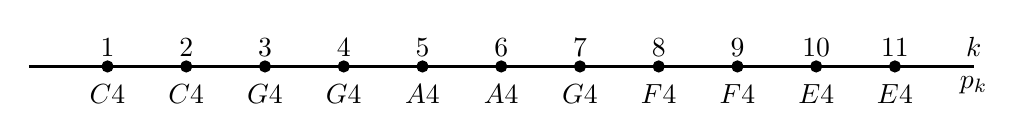
\begin{tikzpicture}
    % Draw number line
    \draw[-, thick] (0,0) -- (12,0) node[below] {$p_k$}  node[above] {$k$};

    % Data
    \foreach \i/\x/\p in {1/C4/1, 2/C4/2, 3/G4/3, 4/G4/4, 5/A4/5, 6/A4/6, 7/G4/7, 8/F4/8, 9/F4/9, 10/E4/10, 11/E4/11} {
      % Draw points and labels
      \filldraw (\i,0) circle (2pt) node[above] {$\p$};
      
      % Draw number scale below the line
      \draw (\i,-0.1) node[below] {$\x$};
    }

  \end{tikzpicture}
  \caption{The first 11 pitches of the Ah vous dirai-je Maman are marked below the 1D axis.}
  \label{subfig:mp}
\end{subfigure}

\vspace{5pt}

\begin{subfigure}{\textwidth}
  \centering
  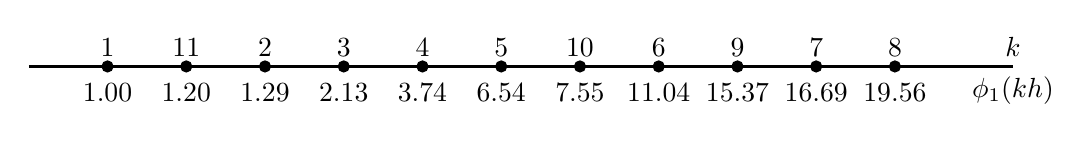
\begin{tikzpicture}
    % Draw number line
    \draw[-, thick] (0,0) -- (12.5,0) node[below] {$\phi_1(kh)$}  node[above] {$k$};

    % Data
    \foreach \i/\x/\p in {1/1.00/1, 2/1.20/11, 3/1.29/2, 4/2.13/3, 5/3.74/4, 6/6.54/5, 7/7.55/10, 8/11.04/6, 9/15.37/9, 10/16.69/7, 11/19.56/8} {
      % Draw points and labels
      \filldraw (\i,0) circle (2pt) node[above] {$\p$};
      
      % Draw number scale below the line
      \draw (\i,-0.1) node[below] {$\x$};
    }

  \end{tikzpicture}
  \caption{The first 11 numerical solution in first component to the system \eqref{eq: re} with initial condition of $(1,1,1)$ are marked below the 1D axis.}
  \label{subfig:traj1}
\end{subfigure}

\vspace{5pt}

\begin{subfigure}{\textwidth}
  \centering
  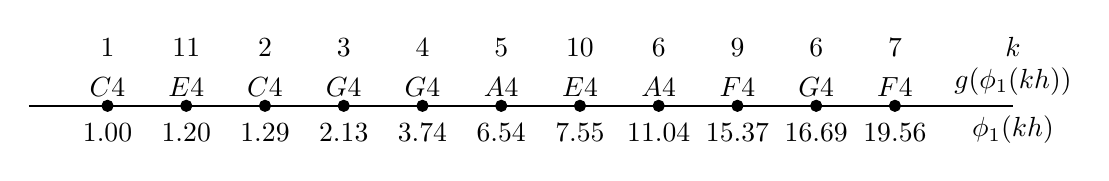
\begin{tikzpicture}
    % Draw number line
    \draw[-, thick] (0,0) -- (12.5,0) node[below] {$\phi_1(kh)$}  node[above] {$g(\phi_1(kh))$} node[above=0.5cm] {$k$};

    % Data
    \foreach \i/\x/\p in {1/1.00/C4, 2/1.20/E4, 3/1.29/C4, 4/2.13/G4, 5/3.74/G4, 6/6.54/A4, 7/7.55/E4, 8/11.04/A4, 9/15.37/F4, 10/16.69/G4, 11/19.56/F4} {
      % Draw points and labels
      \filldraw (\i,0) circle (2pt) node[above] {$\p$};
      
      % Draw number scale below the line
      \draw (\i,-0.1) node[below] {$\x$};
    }
    
    % Display the sequence at each point
    \foreach \i/\x in {1/1, 2/11, 3/2, 4/3, 5/4, 6/5, 7/10, 8/6, 9/9, 10/6, 11/7} {
      \draw (\i,0.5) node[above] {\x};
    }
  \end{tikzpicture}
  \caption{For each component in $\{\phi_1(kh)\}_{k=0}^{10}$, apply the $g(\phi_1(kh))$ mapping.}
  \label{subfig:traj1mp}

\end{subfigure}

\vspace{5pt}

\begin{subfigure}{\textwidth}
  \centering
  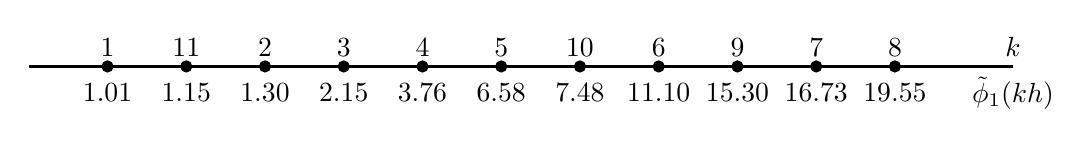
\begin{tikzpicture}
    % Draw number line
    \draw[-, thick] (0,0) -- (12.5,0) node[below] {$\tilde{\phi}_1(kh)$}  node[above] {$k$};

    % Data
    \foreach \i/\x/\p in {1/1.01/1, 2/1.15/11, 3/1.30/2, 4/2.15/3, 5/3.76/4, 6/6.58/5, 7/7.48/10, 8/11.10/6, 9/15.30/9, 10/16.73/7, 11/19.55/8} {
      % Draw points and labels
      \filldraw (\i,0) circle (2pt) node[above] {$\p$};
      
      % Draw number scale below the line
      \draw (\i,-0.1) node[below] {$\x$};
    }

  \end{tikzpicture}
  \caption{The first 11 numerical solution in first component to the system \eqref{eq: re} with new initial condition of $(1.01,1,1)$ are marked below the 1D axis.}
  \label{subfig:traj2}

\end{subfigure}

\vspace{5pt}

\begin{subfigure}{\textwidth}
  \centering
  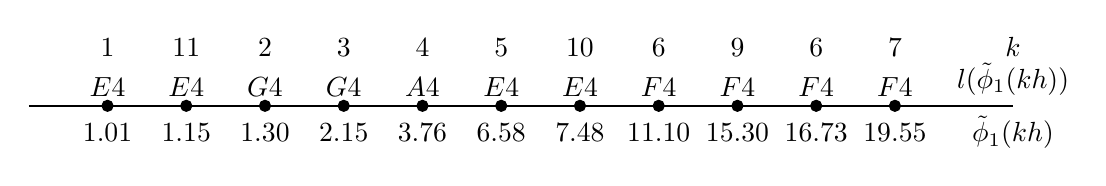
\begin{tikzpicture}
    % Draw number line
    \draw[-, thick] (0,0) -- (12.5,0) node[below] {$\tilde{\phi}_1(kh)$}  node[above] {$l(\tilde{\phi}_1(kh))$} node[above=0.5cm] {$k$};

    % Data
    \foreach \i/\x/\p in {1/1.01/E4, 2/1.15/E4, 3/1.30/G4, 4/2.15/G4, 5/3.76/A4, 6/6.58/E4, 7/7.48/E4, 8/11.10/F4, 9/15.30/F4, 10/16.73/F4, 11/19.55/F4} {
      % Draw points and labels
      \filldraw (\i,0) circle (2pt) node[above] {$\p$};
      
      % Draw number scale below the line
      \draw (\i,-0.1) node[below] {$\x$};
    }
    
    % Display the sequence at each point
    \foreach \i/\x in {1/1, 2/11, 3/2, 4/3, 5/4, 6/5, 7/10, 8/6, 9/9, 10/6, 11/7} {
      \draw (\i,0.5) node[above] {\x};
    }
  \end{tikzpicture}
  \caption{For each component in $\{\tilde{\phi}_1(kh)\}_{k=0}^{10}$, apply the $l(\tilde{\phi}_1(kh))$ mapping.}
  \label{subfig:traj2nmp}

\end{subfigure}

\vspace{5pt}

\begin{subfigure}{\textwidth}
  \centering
  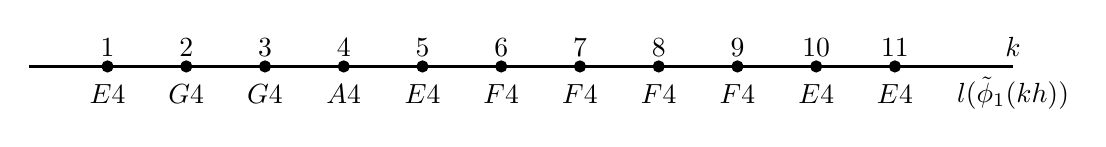
\begin{tikzpicture}
    % Draw number line
    \draw[-, thick] (0,0) -- (12.5,0) node[below] {$l(\tilde{\phi}_1(kh))$}  node[above] {$k$};

    % Data
    \foreach \i/\x/\p in {1/E4/1, 2/G4/2, 3/G4/3, 4/A4/4, 5/E4/5, 6/F4/6, 7/F4/7, 8/F4/8, 9/F4/9, 10/E4/10, 11/E4/11} {
      % Draw points and labels
      \filldraw (\i,0) circle (2pt) node[above] {$\p$};
      
      % Draw number scale below the line
      \draw (\i,-0.1) node[below] {$\x$};
    }
  \end{tikzpicture}
  \caption{The new variation of the first 11 pitches are marked below the 1D axis.}
  \label{subfig:nmp}

\end{subfigure}

\caption{The figure for visualizes how a chaotic mapping method can be used to generate musical variations}
\label{fig:dabby method}
\end{figure}

\subsection{Melodic Variation with Expanded Rhythm Method} 
\label{subsec: melodicvariationwithexpandedrhythm}
In this section, we introduce a method for expanding the rhythm of musical notes, which creates more possibilities for new musical variations. Let $\{p_k\}_{k=0}^{m-1}$ be a sequence of music pitches, we can define a sequence of expanded music pitches $\{p^\prime_k\}_{k=0}^{mq-1}$, where $q$ be a positive integer representing a number of expanded notes for each $p_k$ and $p_k = p^\prime_{kq} = p^\prime_{kq + 1} = \dots = p^\prime_{q(k + 1) - 1}$.

\begin{example}
\label{ex: MV}
Let $ \{p_k\}_{k=0}^{3} = \{ C4, C4, G4, G4 \} $ represent the sequence of music pitches from the music piece Ah vous dirai-je Maman in the first bars, illustrated in Figure \ref{fig:MV1},
Given $q = 4$ represent the number of expanded notes for each $p_k$, we can define a sequence of expanded music pitches 
\[\{p^\prime_k\}_{k=0}^{15} = \{ C4, C4, C4, C4, C4, C4, C4, C4, G4, G4, G4, G4, G4, G4, G4, G4 \}, \] 
illustrated in Figure \ref{fig:MV2}.

\end{example}

\begin{figure}
\centering
\begin{subfigure}{\textwidth}
\centering
\includegraphics[trim=1cm 26.5cm 14.325cm 0.02cm, clip, scale=0.8]{dabby_1.pdf} % trim={left bottom right top}
\caption{The original of Ah vous dirai-je Maman in the first bars.}
\label{fig:MV1} 
\end{subfigure}
\begin{subfigure}{\textwidth}
\centering
\includegraphics[trim=1cm 26.5cm 8.615cm 0.5cm, clip, scale=0.8]{melody_variation.pdf}
\caption{The melodic variation of Ah vous dirai-je, maman in the first bars.}
\label{fig:MV2}
\end{subfigure}
\caption{The original and melodic variation of Ah vous dirai-je Maman.}
\end{figure}

\begin{example}

Consider the sequence $\{p_k\}_{k=0}^{13}$ from Example \ref{ss: mvfacm}, we follow the step mention in Section \ref{ss: mvfacm} to the sequence $\{p^\prime_k\}_{k=0}^{15}$ from Example \ref{ex: MV} by using the initial condition $x(0) = (0.5,0.5,0.5)$ and new trajectory initial condition $\tilde{x}(0) = (0.6,0.5,0.5)$. 
This results in a sequence of new pitches \[ \{l(\tilde{\phi}_1(kh))\}_{k = 0}^{15} = \{C4, G4, D4, A4, A4, E4, F4, F4, F4, F4, E4, G4, D4, C4, C4, C4 \}, \] illustrated in Figure \ref{fig:DabbyER}. Additionally, the visualization of this method illustrated in Figure \ref{fig:dabby method}. The new sequence of musical pitches is significantly different from the original sequence and the changes in pitch are large enough that audience would hear the difference between the original and new notes as much as the change suggests, which makes this method suitable for generating more interesting musical variations.

\end{example}

\begin{figure}
\centering
\includegraphics[trim=1cm 27.5cm 8.65cm 0.5cm, clip, scale=0.8]{dabby_melody_variation.pdf}
\caption{The new variation with melodic variation of Ah vous dirai-je, maman in the first bars, generated by the Initial Condition $(0.6, 0.5, 0.5)$.} 
\label{fig:DabbyER}
\end{figure}

\begin{figure}
\centering

\begin{subfigure}{\textwidth}
  \centering
  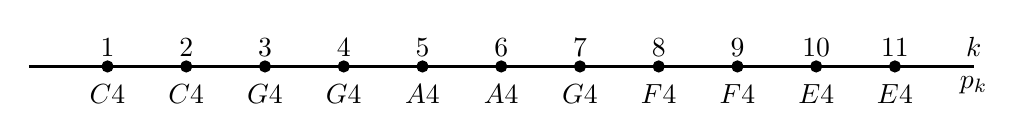
\begin{tikzpicture}
    % Draw number line
    \draw[-, thick] (0,0) -- (12,0) node[below] {$p_k$}  node[above] {$k$};

    % Data
    \foreach \i/\x/\p in {1/C4/1, 2/C4/2, 3/G4/3, 4/G4/4, 5/A4/5, 6/A4/6, 7/G4/7, 8/F4/8, 9/F4/9, 10/E4/10, 11/E4/11} {
      % Draw points and labels
      \filldraw (\i,0) circle (2pt) node[above] {$\p$};
      
      % Draw number scale below the line
      \draw (\i,-0.1) node[below] {$\x$};
    }

  \end{tikzpicture}
  \caption{The first 11 pitches of the Ah vous dirai-je Maman are marked below the 1D axis.}
  \label{subfig2:mp}
\end{subfigure}

\vspace{5pt}

\begin{subfigure}{\textwidth}
  \centering
  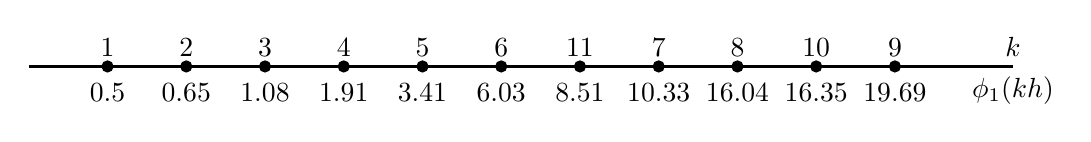
\begin{tikzpicture}
    % Draw number line
    \draw[-, thick] (0,0) -- (12.5,0) node[below] {$\phi_1(kh)$}  node[above] {$k$};

    % Data
    \foreach \i/\x/\p in {1/0.5/1, 2/0.65/2, 3/1.08/3, 4/1.91/4, 5/3.41/5, 6/6.03/6, 7/8.51/11, 8/10.33/7, 9/16.04/8, 10/16.35/10, 11/19.69/9} {
      % Draw points and labels
      \filldraw (\i,0) circle (2pt) node[above] {$\p$};
      
      % Draw number scale below the line
      \draw (\i,-0.1) node[below] {$\x$};
    }

  \end{tikzpicture}
  \caption{The first 11 numerical solution in first component to the system \eqref{eq: re} with initial condition of $(0.5,0.5,0.5)$ are marked below the 1D axis.}
  \label{subfig2:traj1}
\end{subfigure}

\vspace{5pt}

\begin{subfigure}{\textwidth}
  \centering
  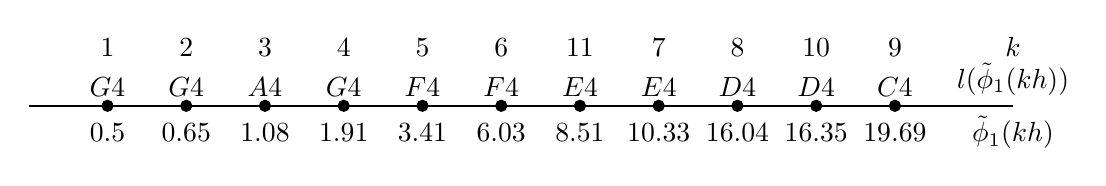
\begin{tikzpicture}
    % Draw number line
    \draw[-, thick] (0,0) -- (12.5,0) node[below] {$\tilde{\phi}_1(kh)$}  node[above] {$l(\tilde{\phi}_1(kh))$} node[above=0.5cm] {$k$};

    % Data
    \foreach \i/\x/\p in {1/0.5/G4, 2/0.65/G4, 3/1.08/A4, 4/1.91/G4, 5/3.41/F4, 6/6.03/F4, 7/8.51/E4, 8/10.33/E4, 9/16.04/D4, 10/16.35/D4, 11/19.69/C4} {
      % Draw points and labels
      \filldraw (\i,0) circle (2pt) node[above] {$\p$};
      
      % Draw number scale below the line
      \draw (\i,-0.1) node[below] {$\x$};
    }
    
    % Display the sequence at each point
    \foreach \i/\x in {1/1, 2/2, 3/3, 4/4, 5/5, 6/6, 7/11, 8/7, 9/8, 10/10, 11/9} {
      \draw (\i,0.5) node[above] {\x};
    }
  \end{tikzpicture}
  \caption{For each component in $\{\phi_1(kh)\}_{k=0}^{10}$, apply the $g(\phi_1(kh))$ mapping.}
  \label{subfig2:traj1mp}

\end{subfigure}

\vspace{5pt}

\begin{subfigure}{\textwidth}
  \centering
  \small{
  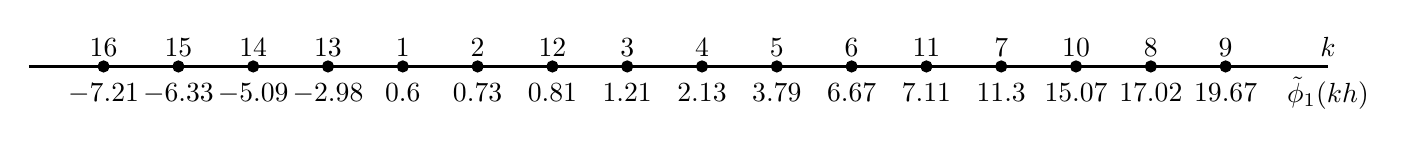
\begin{tikzpicture}
    % Draw number line
    \draw[-, thick] (0,0) -- (16.5,0) node[below] {$\tilde{\phi}_1(kh)$}  node[above] {$k$};

    % Data
    \foreach \i/\x/\p in {1/-7.21/16, 2/-6.33/15, 3/-5.09/14, 4/-2.98/13, 5/0.6/1, 6/0.73/2, 7/0.81/12, 8/1.21/3, 9/2.13/4, 10/3.79/5, 11/6.67/6, 12/7.11/11, 13/11.3/7, 14/15.07/10, 15/17.02/8, 16/19.67/9} {
      % Draw points and labels
      \filldraw (\i*0.95,0) circle (2pt) node[above] {$\p$};
      
      % Draw number scale below the line
      \draw (\i*0.95,-0.1) node[below] {$\x$};
    }

  \end{tikzpicture}}
  \caption{The first 16 numerical solution in first component to the system \eqref{eq: re} with new initial condition of $(0.6,0.5,0.5)$ are marked below the 1D axis.}
  \label{subfig2:traj2}

\end{subfigure}

\vspace{5pt}

\begin{subfigure}{\textwidth}
  \centering
  \small{
  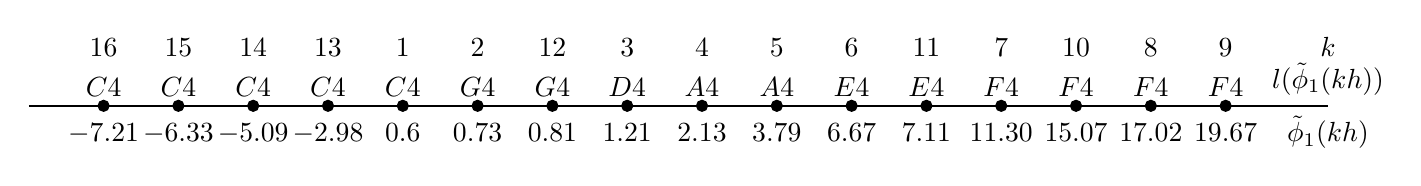
\begin{tikzpicture}
    % Draw number line
    \draw[-, thick] (0,0) -- (16.5,0) node[below] {$\tilde{\phi}_1(kh)$}  node[above] {$l(\tilde{\phi}_1(kh))$} node[above=0.5cm] {$k$};

    % Data
    \foreach \i/\x/\p in {1/-7.21/C4, 2/-6.33/C4, 3/-5.09/C4, 4/-2.98/C4, 5/0.6/C4, 6/0.73/G4, 7/0.81/G4, 8/1.21/D4, 9/2.13/A4, 10/3.79/A4, 11/6.67/E4, 12/7.11/E4, 13/11.30/F4, 14/15.07/F4, 15/17.02/F4, 16/19.67/F4} {
      % Draw points and labels
      \filldraw (\i*0.95,0) circle (2pt) node[above] {$\p$};
      
      % Draw number scale below the line
      \draw (\i*0.95,-0.1) node[below] {$\x$};
    }
    
    % Display the sequence at each point
    \foreach \i/\x in {1/16, 2/15, 3/14, 4/13, 5/1, 6/2, 7/12, 8/3, 9/4, 10/5, 11/6, 12/11, 13/7, 14/10, 15/8, 16/9} {
      \draw (\i*0.95,0.5) node[above] {\x};
    }
  \end{tikzpicture}}
  \caption{For each component in $\{\tilde{\phi}_1(kh)\}_{k=0}^{15}$, apply the $l(\tilde{\phi}_1(kh))$ mapping.}
  \label{subfig2:traj2nmp}

\end{subfigure}

\vspace{5pt}

\begin{subfigure}{\textwidth}
  \centering
  \small{
  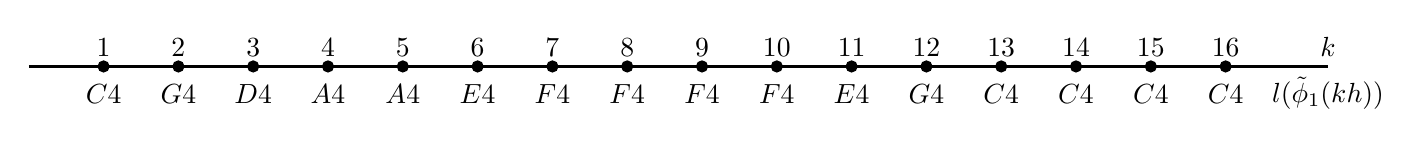
\begin{tikzpicture}
    % Draw number line
    \draw[-, thick] (0,0) -- (16.5,0) node[below] {$l(\tilde{\phi}_1(kh))$}  node[above] {$k$};

    % Data
    \foreach \i/\x/\p in {1/C4/1, 2/G4/2, 3/D4/3, 4/A4/4, 5/A4/5, 6/E4/6, 7/F4/7, 8/F4/8, 9/F4/9, 10/F4/10, 11/E4/11, 12/G4/12, 13/C4/13, 14/C4/14, 15/C4/15, 16/C4/16} {
      % Draw points and labels
      \filldraw (\i*0.95,0) circle (2pt) node[above] {$\p$};
      
      % Draw number scale below the line
      \draw (\i*0.95,-0.1) node[below] {$\x$};
    }

  \end{tikzpicture}}
  \caption{The new variation of the first 16 pitches are marked below the 1D axis.}
  \label{subfig2:nmp}

\end{subfigure}

\caption{The figure for visualizes how a chaotic mapping with melodic variation method can be used to generate musical variations}
\label{fig2:dabbymv method}
\end{figure}

\section{Discussion}
\label{sec: discussion}
This section discusses the potential of combining musical variations from a chaotic mapping and melodic variation with expanded rhythm method for generating musical variations. We will also analyze the impact of this approach on the resulting variations in other sheet music. For convenience, we will refer to this combination of methods as the combined approach throughout this section. 

\subsection{Strengths of the Combined Approach}

The combined approach shows potential in generating interesting musical variations, as shown in the new variations with melodic variation of Pachelbel's Canon \cite{pachelbel_canon_2005} (Figure \ref{fig:NCND}) compared to the original melody (Figure \ref{fig:OCND}).

This method appears to be particularly effective for pieces with a larger range of musical pitches. The additional pitches provide more material for the chaotic mapping and melodic variation techniques to manipulate, leading to richer and more diverse variations.

\begin{figure}
\begin{subfigure}{\textwidth}
\centering
\includegraphics[trim=1cm 26.5cm 1cm 0.5cm, clip, scale=0.8]{Original_CND.pdf}
\caption{The original of Pachelbel's Canon in the first 10 bars.} 
\label{fig:OCND}
\end{subfigure}
\begin{subfigure}{\textwidth}
\centering
\includegraphics[trim=1cm 20.3cm 1cm 0.5cm, clip, scale=0.8]{New_CND.pdf}
\caption{The new variation with melodic variation of Pachelbel's Canon in the first 10 bars (including 2 additional bars at the end of the 10th bar).} 
\label{fig:NCND}
\end{subfigure}
\caption{The combined approach with Pachelbel's Canon in the first 10 bars.} 
\label{fig: exam1}
\end{figure}

\subsection{Weaknesses of the Combined Approach}

Let's consider the sheet music A Thousand Miles \cite{carlton2009thousandmiles} illustrated in Figure \ref{fig:OATM} and a new variation deriving from melodic variation illustrated in Figure \ref{fig:NATM}. This result shows that using sheet music with too many musical note durations can lead to new variations with melodies that are difficult to play and listen to. This is a major weakness of this method.

\begin{figure}
\begin{subfigure}{\textwidth}
\centering
\includegraphics[trim=1cm 26.5cm 1cm 0.5cm, clip, scale=0.8]{Original_ATM.pdf}
\caption{The original of Vanessa Carlton - A Thousand Miles in the first 3 bars.} 
\label{fig:OATM}
\end{subfigure}
\begin{subfigure}{\textwidth}
\centering
\includegraphics[trim=1cm 23.75cm 1cm 0.5cm, clip, scale=0.8]{New_ATM.pdf}
\caption{The new variation with melodic variation of Vanessa Carlton - A Thousand Miles in the first 3 bars.} 
\label{fig:NATM}
\end{subfigure}
\caption{The combined approach with A Thousand Miles in the first 3 bars.} 
\label{fig: exam2}
\end{figure}

\subsection{Limitations and Considerations}

Further evaluation with a wider range of musical pieces is necessary to determine the generalizability of these observations. The effectiveness of the combined approach might vary depending on the musical style and characteristics of the original piece.

The computational complexity of the chaotic mapping technique should also be considered. While it offers a powerful approach for variation, it might require more processing power compared to simpler melodic variation methods.

\subsection{Future Directions}

Exploring different parameters and configurations within the chaotic mapping and melodic variation techniques could potentially lead to a wider range of variation styles and outcomes.

Investigating methods for user control over the variation process would be valuable. This could allow musicians to tailor the generated variations to their specific creative goals.

Integrating this combined approach into music composition tools could provide composers with a valuable tool for generating new musical ideas and exploring creative possibilities.

\section{Conclusion}
\label{sec: conclusion}
The proposed method, leveraging the power of chaotic systems, offers a promising approach to music composition, addressing the limitations of existing AI techniques and providing composers with a tool to generate novel, unpredictable, and diverse musical compositions while reducing computational resource demands. This method has the potential to stimulate creativity, alleviate composer's burnout, and expand the boundaries of musical expression, paving the way for a new era of music creation driven by chaos and innovation.

\printbibliography

\end{document}